\documentclass[a4paper,12pt]{book}


\usepackage[hidelinks]{hyperref}
\usepackage[margin=1in]{geometry}
\usepackage{mdframed}
\usepackage{lipsum}
\usepackage{amsthm}
\usepackage[normalem]{ulem}
\usepackage{pgfplots,pgf-pie}
\usepackage{wrapfig}
\usepackage{booktabs}
 
\theoremstyle{definition}
\newtheorem{definition}{Definition}[section]

\mdfdefinestyle{MyFrame}{%
    linecolor=black,
    outerlinewidth=2pt,
    %roundcorner=20pt,
    innertopmargin=4pt,
    innerbottommargin=4pt,
    innerrightmargin=4pt,
    innerleftmargin=4pt,
        leftmargin = 4pt,
        rightmargin = 4pt
    %backgroundcolor=gray!50!white}
        }

\newmdtheoremenv{theo}{Theorem}

\pgfplotsset{width=7cm,compat=1.16}

\hypersetup{
  linktoc=all,
  linkcolor=black
}

\title{2020 AP Statistics Review}
\author{Bryan Li}
\date{\today}

\begin{document}

\begingroup
  \let\newpage\relax%
  \maketitle
\endgroup
\large{\tableofcontents}


\chapter{Working with Data}
\section{Data, what is it?}
In this section, we'll be working with data. Remember, data are \textbf{values}
along with their \textbf{context}.

\subsection{Context}
When describing the context of data, it is important to consider the W's
\begin{itemize}
  \item Who? - Who was the data collected from? 
  \item What? - The variables recorded from each experimental unit, and the unit of measurement.
What type is the variable? Quantitative or categorical?
  \item When? - When was the data collected?
  \item Where? - Where was the data collected?
  \item Why? - Why was the data collected?
  \item How? - How was the data collected?
\end{itemize}
Data without context is useless. For example, consider:
\begin{center}
  1.2, 3.7, 4.4, 2.2
\end{center}
Are these data? No. These are just numbers without any context. Numbers without any context mean nothing.

\subsection{Types of Data}
There are two types of data. These include \emph{categorical} and \emph{quantitative} data.
These two types of data must be expressed differently.

\begin{mdframed}
  \begin{definition}{\textbf{\underline{Categorical Variable:}}}
    A categorical variable is a variable that can take on one of a limited amount
  of possible values. Individuals are assigned to a group by some qualitative property.
  Examples: race, sex, eye color.
  \end{definition}
\end{mdframed}

\begin{mdframed}
  \begin{definition}{\textbf{\underline{Quantitative Variable:}}}
    A quantitative variable is a variable that is measured on a numeric scale.
    Examples: age, height, weight.
  \end{definition}
\end{mdframed}

\section{Displaying Data}
When displaying data, it is important to follow the \emph{area principle}.

\begin{mdframed}
  \begin{definition}{\textbf{\underline{Area Principle:}}}
    The area principle states that the area of a graph should equal the 
    magnitude of the data it represents.
  \end{definition}
\end{mdframed}
Be careful, as many 3D graph types can violate the area principle.

\subsection{Displaying Categorical Data}
Categorical data are displayed primarily with 2 types of visual charts: Bar graphs and pie charts. It can
also be expressed with a frequency table, like the one in Figure 1.1.


\begin{figure}[h!]
  
  \centering
  \caption{An example frequency table}
  Sex of Respondents\\
  \begin{tabular}{@{}cccc@{}}
    \toprule
    Sex       & Male & Female & Total \\ \midrule
    Frequency & 13   &   10   & 23     \\ \bottomrule
  \end{tabular}
  
\end{figure}


\subsubsection{Bar Graphs}
There are many types of bar graphs. They include normal bar graphs, frequency bar graphs, and stacked
bar graphs. Below are examples of different types of bar graphs. \textbf{It is important
that the bars do not touch each other. This signifies the bars are ordered. Categorical
variables cannot be ordered in a meaningful way, so this is wrong.}
\begin{itemize}
  \item Normal Bar Graph: Displays the total number of cases in each category.
  \item Relative Frequency Bar Graph: Displays the relative frequency (percentage or decimal)
of each category. All relative frequencies add up to 100\%, or 1.
  \item Stacked Bar Graph: Shows comparisons between categories of data.
\end{itemize}

\begin{figure}[bp!]
  
  \centering
  \caption{An example of a bar graph}
  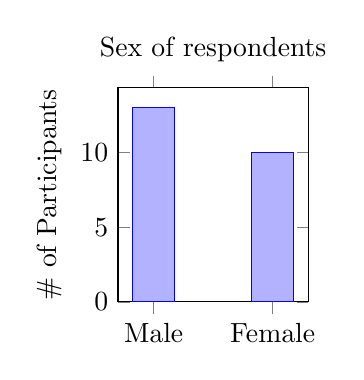
\begin{tikzpicture}
    \begin{axis}[
      title={Sex of respondents},
      ybar,
      bar width=15pt,
      enlarge x limits=0.3,
      ylabel={\# of Participants},
      symbolic x coords={Male,Female},
      xtick=data,
      ymin=0,
      width=4cm,
      height=4.3cm,
    ]
    \addplot coordinates {(Male,13) (Female,10)};
    \end{axis}
  \end{tikzpicture}

\end{figure}
\begin{figure}[bp!]

  \centering
  \caption{An example of a relative frequency bar graph}
  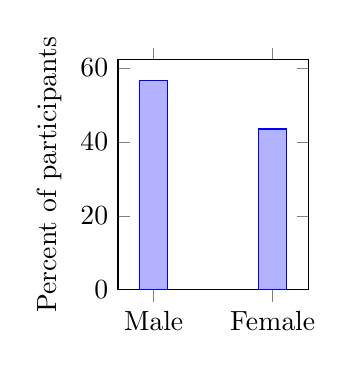
\begin{tikzpicture}
    \begin{axis}[
      ybar,
      enlarge x limits=0.3,
      ylabel={Percent of participants},
      symbolic x coords={Male,Female},
      xtick=data,
      ymin=0,
      width=4cm,
      height=4.5cm,
    ]
    \addplot coordinates {(Male,56.52) (Female,43.48)};
    \end{axis}
  \end{tikzpicture}

\end{figure}
\begin{figure}[bp!]

  \centering
  \caption{An example of a stacked bar graph}
  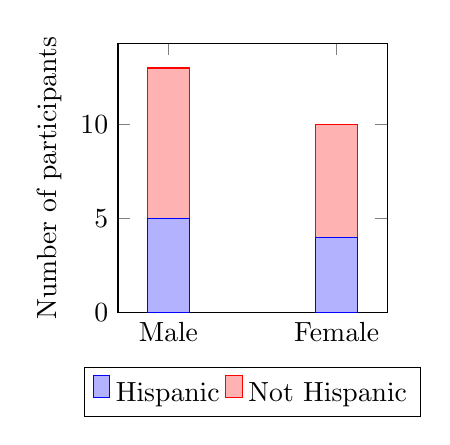
\begin{tikzpicture}
    \begin{axis}[
      ybar stacked,
      bar width=15pt,
      enlarge x limits=0.3,
      ylabel={Number of participants},
      symbolic x coords={Male,Female},
      xtick=data,
      ymin=0,
      width=5cm,
      height=5cm,
      legend style={at={(0.5,-0.20)},
      anchor=north,legend columns=-1},
    ]
    \addplot+[ybar] plot coordinates {(Male,5) (Female,4)};
    \addplot+[ybar] plot coordinates {(Male,8) (Female,6)};
    \legend{\strut Hispanic, \strut Not Hispanic}

    \end{axis}
  \end{tikzpicture}
\end{figure}
\clearpage

\subsubsection{Pie Charts}
While bar graphs are great for looking at numerical values, pie charts can 
be useful when determining the percent composition of the categories. Below
is an example of a pie chart. 

\begin{wrapfigure}{r}{0.4\textwidth}
  \caption{An example pie chart}
  \begin{small}
    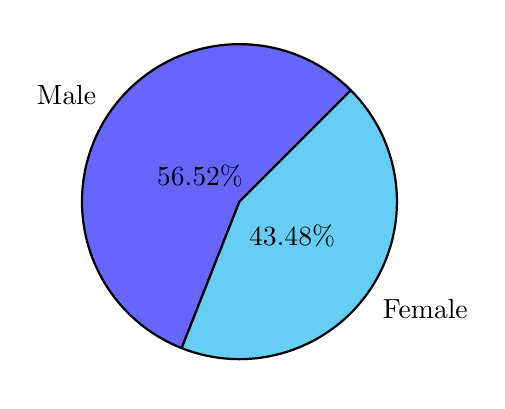
\begin{tikzpicture}
    
    \pie [rotate = 45,radius=2]{56.52/Male, 43.48/Female}
    \end{tikzpicture}
  \end{small}
\end{wrapfigure}

As you can see, the pie chart does not violate the area principle. Each "slice"
of a pie chart grows in size. Polar area charts, which are similar to pie charts,
do not obey the area principle. You should also see that the sum of the relative frequencies
equals 100\%, or 1.

\subsection{Displaying Quantitative Data}
Displaying quantitative data is a bit different from displaying categorical data.
Display methods are typically box-and-whisker plots, histograms, and stem plots.



\end{document}